\documentclass[aspectratio=169]{beamer}
\beamertemplatenavigationsymbolsempty
\usepackage[utf8]{inputenc}
\usepackage[T1]{fontenc}
\usepackage{bm}
\usepackage{listings}
\usepackage{amsmath, amssymb}
\usepackage{multimedia}
\usepackage{booktabs}
\usepackage{tikz}
\usepackage{graphicx}
\usetikzlibrary{positioning, arrows.meta}
\usepackage{tabularx}
\usepackage{colortbl}
\usepackage{array}
\usepackage{xcolor}
\usepackage{pifont}
\usepackage{draftfigure}

% ====== Macros ======
\newcommand{\cmark}{\textcolor{green!60!black}{\ding{51}}}
\newcommand{\xmark}{\textcolor{red!70!black}{\ding{55}}}

% ====== Listings Setup ======
\lstset{
    basicstyle=\ttfamily\tiny,
    breaklines=true,
    frame=single,
    showstringspaces=false
}

\usetheme{Madrid}
\usecolortheme{beaver}

\title[Power System LLM]{Weekly Report}
\author{Yifei Xu}
\institute{New York University}
\date{\today}

\begin{document}
\maketitle
% ------------------------------------------------
\begin{frame}{Problem Setting}
\textbf{Setting.} We run conventional fundamental-frequency WLS State Estimation (SE) using traditional SCADA-like measurements.
When abnormal harmonics exist, the fundamental-only measurement model becomes inconsistent.

\vspace{0.5em}
\textbf{Goal.} Design an operational pipeline:
\begin{enumerate}
  \item Run fundamental WLS-SE.
  \item Trigger a \textbf{harmonic-state-estimation (HSE)} module when WLS residual statistics indicate an abnormal harmonic condition.
  \item Use HSE to (i) identify the most likely harmonic source location(s) and (ii) estimate harmonic voltage states.
\end{enumerate}

\vspace{0.6em}
\textbf{Key observation from experiments.} With legacy SCADA noise levels, WLS residual tests become reliably sensitive only when voltage THD is \emph{severe} (around $\gtrsim 10\%$).
\end{frame}

% ------------------------------------------------
\begin{frame}{Pipeline Overview: WLS $\rightarrow$ Trigger $\rightarrow$ HSE}
\begin{center}
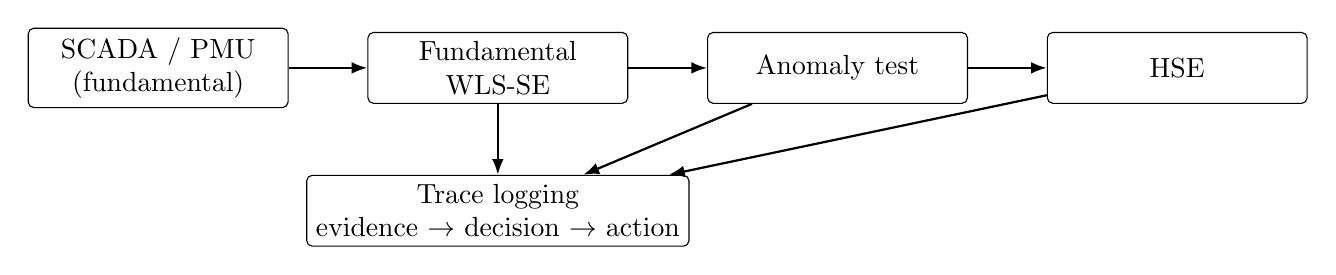
\begin{tikzpicture}[
  node distance=9mm and 10mm,
  box/.style={draw, rounded corners=2pt, align=center, minimum width=3.3cm, minimum height=0.9cm},
  arrow/.style={-{Latex[length=2mm]}, thick}
]
\node[box] (meas) {SCADA / PMU\\(fundamental)};
\node[box, right=of meas] (wls) {Fundamental\\WLS-SE};
\node[box, right=of wls] (test) {Anomaly test};
\node[box, right=of test] (hse) {HSE};
\node[box, below=of wls] (log) {Trace logging\\evidence $\rightarrow$ decision $\rightarrow$ action};

\draw[arrow] (meas) -- (wls);
\draw[arrow] (wls) -- (test);
\draw[arrow] (test) -- (hse);
\draw[arrow] (wls) -- (log);
\draw[arrow] (test) -- (log);
\draw[arrow] (hse) -- (log);
\end{tikzpicture}
\end{center}

\vspace{0.2em}
\small
The trigger is a \emph{gate}: HSE is only run when WLS indicates abnormal model mismatch.
\end{frame}


% ------------------------------------------------
\begin{frame}{Why WLS Needs THD $\gtrsim 10\%$ to Trigger}
With legacy SCADA, harmonic effects often leak into measurements as:
\begin{itemize}
  \item \textbf{RMS magnitude bias:} $|V|_{\mathrm{RMS}} = |V_1|\sqrt{1+\mathrm{THD}^2}$,
  \item weak or indirect impacts on MW/MVar channels.
\end{itemize}

\vspace{0.4em}
Because RMS bias scales approximately with $\mathrm{THD}^2$, the induced deviation is small for moderate THD and becomes pronounced at high THD:
\[
\sqrt{1+\mathrm{THD}^2}-1 \approx \frac{\mathrm{THD}^2}{2}.
\]
For example, THD $=10\%$ yields $\approx 0.5\%$ RMS magnitude increase (often several $\sigma$ for voltage meas), while THD $=2\%$ yields only $\approx 0.02\%$.

\small
\textbf{Note:} Normal planning limits at HV are much lower (e.g., 1.5--2.5\% at 69--161 kV and 1.5\% above 161 kV), so THD $\gtrsim 10\%$ represents \emph{severe abnormality}.
\end{frame}

% ------------------------------------------------
\begin{frame}{When Can Voltage THD Exceed 10\%? (Abnormal Resonance Scenarios)}
\textbf{Main justification: resonance amplification.}
A common pathway to extreme voltage distortion is harmonic resonance involving:
\begin{itemize}
  \item shunt capacitor banks / power-factor correction capacitors,
  \item system (line/cable) capacitance,
  \item network impedance changes under contingencies (line outages, switching).
\end{itemize}

\vspace{0.4em}
\textbf{Mechanism (high-level).}
At a specific harmonic order (e.g., 5th or 7th), the network's driving-point impedance can become large (or exhibit resonance),
so a harmonic current injection produces a much larger harmonic voltage:
\[
V(h) \approx Z_{\mathrm{th}}(h)\, I(h) \;\;\Rightarrow\;\; \text{large }|Z_{\mathrm{th}}(h)| \text{ yields large } |V(h)|.
\]

\vspace{0.4em}
\textbf{Evidence from case studies.}
\begin{itemize}
  \item Transmission case studies report $V_{\mathrm{THD}}>10\%$ on a transmission capacitor bank under line outage conditions.\footnote{\url{https://powerquality.blog/2021/02/25/case-studies-of-harmonic-problems-analysis-solutions-on-transmission-systems/}}
  \item A detailed harmonic case study shows a highest voltage distortion of \emph{14.1\%} (unacceptable) at a bus prior to mitigation.\footnote{\url{https://web.ecs.baylor.edu/faculty/grady/understanding_power_system_harmonics_grady_april_2012.pdf}}
\end{itemize}
\end{frame}


% ------------------------------------------------
\begin{frame}{HSE Model: Frequency-Domain Network Equations}
For each harmonic order $h \in \mathcal{H}$ (e.g., $\{5,7,11,13,\dots\}$), we build a harmonic admittance model:
\[
Y(h)\,V(h)=I(h),
\]
where:
\begin{itemize}
  \item $Y(h)$ uses frequency-scaled line/transformer parameters and shunt elements,
  \item $V(h)$ are bus harmonic voltage phasors,
  \item $I(h)$ are harmonic current injections (sources).
\end{itemize}

\vspace{0.4em}
\textbf{HSE objective.} Estimate $V(h)$ from limited harmonic measurements.
\end{frame}

% ------------------------------------------------
\begin{frame}{HSE Implementation After Trigger (Single-Source Scan)}
In our triggered experiments, we assume \textbf{one dominant harmonic source} among candidate buses:
\[
I(h)=e_s\,I_s(h),
\]
where $s$ is the source bus and $I_s(h)$ is the complex injection at harmonic $h$.

\vspace{0.4em}
With slack harmonic voltage fixed (often $V_{\text{slack}}(h)=0$), we work with the reduced network:
\[
V_u(h) = Z_{uu}(h)\,I_u(h), \quad Z_{uu}(h)=Y_{uu}(h)^{-1}.
\]
For measured harmonic voltages at meter buses $M$:
\[
V_M(h) \approx Z_{M,s}(h)\,I_s(h) + \varepsilon.
\]

\vspace{0.4em}
\textbf{Estimation by candidate scan.}
For each candidate $s$ and harmonic $h$, estimate $I_s(h)$ by (complex) least squares and compute a weighted fit error.
Sum errors across harmonics and pick the minimum-score bus:
\[
s^\star = \arg\min_s \sum_{h\in\mathcal{H}} \mathrm{SSE}(h,s).
\]

\vspace{0.3em}
\small
This is compatible with HSE goals (source location + harmonic state reconstruction) and is a practical special case of broader HSE methods.\footnote{\url{https://users.ece.cmu.edu/~hliao/paper/liao-hse-pwrs.pdf}}
\end{frame}

% % ------------------------------------------------
% \begin{frame}{Generalization: Sparse Multi-Source HSE (If Needed)}
% If multiple harmonic sources may be present, a common assumption is \textbf{sparsity}:
% only a small number of buses inject significant harmonic currents.

% \vspace{0.4em}
% Then HSE can be posed as a constrained sparse recovery problem over $I(h)$:
% \[
% \min \|I(h)\|_1 \quad \text{s.t.} \quad \|V_M(h) - Z_{M}(h)I(h)\|_2 \le \epsilon,
% \]
% or an equivalent optimization over stacked harmonics, potentially solved efficiently.

% \vspace{0.4em}
% \small
% Sparsity-based observability and estimation for underdetermined HSE is developed and validated on IEEE-14 in Liao (TPWRS).\footnote{\url{https://users.ece.cmu.edu/~hliao/paper/liao-hse-pwrs.pdf}}
% \end{frame}

% ------------------------------------------------
\begin{frame}{Performance Verification After HSE Trigger}
We evaluate HSE performance at three levels.

\vspace{0.4em}
\textbf{1) Source localization (classification).}
\begin{itemize}
  \item Top-1 accuracy: $\mathbb{1}\{s^\star = s_{\mathrm{true}}\}$
  \item Rank of true source in candidate list; Top-$k$ accuracy
  \item Confidence: score gap ratio $\mathrm{score}_2/\mathrm{score}_1$ (larger is better)
\end{itemize}

\vspace{0.4em}
\textbf{2) Harmonic state accuracy (regression, simulation).}
\begin{itemize}
  \item Voltage state error per harmonic: $\mathrm{RMSE}_V(h)=\sqrt{\frac{1}{N}\sum_i|V_i^{\hat{}}(h)-V_i(h)|^2}$
  \item Injection error per harmonic (magnitude/angle/complex relative error) for $I_s(h)$
\end{itemize}

\vspace{0.4em}
\textbf{3) Statistical fit (measurement consistency).}
\begin{itemize}
  \item Hold-out validation on harmonic meters: whitened SSE/dof $\approx 1$ indicates consistent fit
  \item Optional $p$-value using $\chi^2$ approximation on hold-out residual energy
\end{itemize}

\end{frame}

% ------------------------------------------------
\begin{frame}{Derived Metric: THD Map Reconstruction}
From estimated harmonic voltages, compute bus-wise voltage THD:
\[
\mathrm{THD}_V(i)=\frac{\sqrt{\sum_{h>1}|V_i(h)|^2}}{|V_i(1)|}.
\]
Then evaluate:
\begin{itemize}
  \item THD RMSE over buses,
  \item max THD error at ``hot'' buses,
  \item spatial consistency: does the THD map peak near the identified source and propagate realistically?
\end{itemize}

\vspace{0.3em}
\small
This THD definition aligns with standard power-quality definitions (IEEE 1459 framework).\footnote{\url{https://thece.eu/wp-content/uploads/2020/07/1459-2010.pdf}}
\end{frame}

\begin{frame}{Experimental Results: HSE Validation (10\% THD Case)}
    We validated the HSE module on the IEEE 14-bus benchmark with simulated harmonic injections (10--20\% THD).
    
    \vspace{0.5em}
    \textbf{Estimation Accuracy (vs Ground Truth):}
    \begin{itemize}
      \setlength\itemsep{0.3em}
      \item \textbf{Source Injection Error:} \textcolor{green!40!black}{\textbf{1.10\%}} 
      \par {\footnotesize (Average magnitude error across harmonic orders)}
      
      \item \textbf{Voltage State Error:} \textcolor{green!40!black}{\textbf{0.72\%}}
      \par {\footnotesize (Global relative RMSE across all buses)}
      
      \item \textbf{THD Estimation Accuracy:} \textcolor{green!40!black}{\textbf{0.02\%}}
      \par {\footnotesize (Mean Absolute Error in THD percentage points. Example: True 7.17\%, Est 7.14\%)}
    \end{itemize}
    
    \vspace{0.6em}
    \textbf{Conclusion:} Once triggered, the HSE module provides high-fidelity recovery of the harmonic state and accurate localization of the source.
\end{frame}

\begin{frame}[fragile]{Sample SFT Trace: Harmonic Diagnosis Agent}
    \footnotesize
    \textbf{Scenario}: Agent receives SCADA data with underlying harmonic distortion (Source: Bus 11).
    
    \vspace{0.2cm}
    
    \begin{itemize}
        \setlength\itemsep{0.2cm}
        
        \item[\textbf{User}] \textit{Request}: ``Diagnose grid state.'' (SCADA $z$ vector attached)
        
        \item[\textbf{Agent}] \textit{Step 1: State Estimation}
        \begin{itemize}
            \item \textbf{Tool Call}: \texttt{wls\_from\_path(case\_path='case14', z=[...])}
            \item \textbf{Tool Output}: \texttt{\{success: true, r: [9.08, 0.45, ...]\}}
        \end{itemize}
        
        \item[\textbf{Agent}] \textit{Reasoning}: 
        ``WLS residual sum $J=60980.3$ exceeds threshold $118.8$. Suspecting harmonic interference. Initiating Harmonic State Estimation.''
        
        \item[\textbf{Agent}] \textit{Step 2: Harmonic Analysis}
        \begin{itemize}
            \item \textbf{Tool Call}: \texttt{run\_hse\_from\_path(harmonic\_measurements=[...])}
            \item \textbf{Tool Output}: \texttt{\{best\_candidate: 11, max\_thd: 25.12\%, ...\}}
        \end{itemize}
        
        \item[\textbf{Agent}] \textit{Final Response}:
        \begin{tcolorbox}[colback=green!5!white,colframe=green!50!black, boxrule=0.5pt, sharp corners=south]
            \textbf{Diagnosis}: Harmonic source identified.\\
            \textbf{Location}: Bus 11 \quad \textbf{Est. THD}: 25.1\% \quad \textbf{Confidence}: High
        \end{tcolorbox}
    \end{itemize}
\end{frame}

% % ------------------------------------------------
% \begin{frame}{References (URLs)}
% \footnotesize
% \begin{itemize}
%   \item Grady, \emph{Understanding Power System Harmonics} (case study with THD$_V$ up to 14.1\%):\\
%   \url{https://web.ecs.baylor.edu/faculty/grady/understanding_power_system_harmonics_grady_april_2012.pdf}
%   \item Transmission case studies noting $V_{\mathrm{THD}}>10\%$ on capacitor bank under line outage conditions:\\
%   \url{https://powerquality.blog/2021/02/25/case-studies-of-harmonic-problems-analysis-solutions-on-transmission-systems/}
%   \item IEEE 519 voltage THD planning limits (summary table):\\
%   \url{https://www.mirusinternational.com/downloads/White\%20Paper\%20-\%20IEEE\%20Std\%20519-2014\%20Harmonic\%20Limits.pdf}
%   \item Liao, \emph{Power System Harmonic State Estimation and Observability via Sparsity Maximization}:\\
%   \url{https://users.ece.cmu.edu/~hliao/paper/liao-hse-pwrs.pdf}
%   \item Meliopoulos et al., \emph{Power system harmonic state estimation} (overview + performance framing):\\
%   \url{https://www.osti.gov/biblio/7054602}
%   \item IEEE 1459 (power quantities / THD framework):\\
%   \url{https://thece.eu/wp-content/uploads/2020/07/1459-2010.pdf}
% \end{itemize}
% \end{frame}
\end{document}